\documentclass[a4paper, 11pt]{article}
\usepackage{graphicx}
\usepackage{amsmath}
\usepackage{hyperref}
\usepackage{cite}
\usepackage{color}
\usepackage{subcaption} 


% Lengths and indenting
\setlength{\textwidth}{16.5cm}
\setlength{\marginparwidth}{1.5cm}
\setlength{\parindent}{0cm}
\setlength{\parskip}{0.15cm}
\setlength{\textheight}{22cm}
\setlength{\oddsidemargin}{0cm}
\setlength{\evensidemargin}{\oddsidemargin}
\setlength{\topmargin}{0cm}
\setlength{\headheight}{0cm}
\setlength{\headsep}{0cm}

\renewcommand{\familydefault}{\sfdefault}

\renewcommand{\labelenumii}{\theenumii}
\renewcommand{\theenumii}{\theenumi.\arabic{enumii}.}

\title{Agent-Based Modelling Project\\
Modelling of Language Competition in Bilingual Society}
\author{Simulation of Language Competition: Coexistence and Dominance of a Language in Social Network}
 \author{Michael King Nam Yip, Zichao Han}
\date{}

\begin{document}
\maketitle
% \begin{center}
\section{Introduction}
The idea of our project arises from the language competition between the dialect Cantonese and the official language Mandarin, which is a controversial issue happening in Hong Kong. \cite{WinNT} Hong Kong citizens are wary of the language shift from their mother tongue Cantonese to Mandarin in recent years, and some fears that the dialect will soon become extinct. This shift is caused by, for instance, polictical pressure and increasing prestige of Mandarin and the increasing number of immigrants who are Mandarin speakers. This is just one example of language competition. In fact, language competition has long existed worldwide and is a notable issue in linguistic or sociological field. 

Apart from political or educational factors, the usage of a language is strongly affected by the interactions between individuals within a society. \cite{patriarca2012modeling} The switch of language use behaves similarly to how opinion change and it resembles the opinion dynamics described in this course. Therefore, language competition can be well simulated and described by an agent-based model. In this project, we will observe the language dynamics of the choices made by the agents, i.e. whether agents will stick with the current language or switch to another language, using an agent-based model. From it we will examine how two similar languages compete in a bilingual society and in what circumstances will a language exist or extinct. 

As in some linguistic study, the change in language use is believed to be related to the social structure in the society. Social network is suggested to be an important factor related to the existance of a language\cite{castello2008modelling}. Here in our project we would like to justify and examine this. Thus, we will place the model in different social network settings and determine whether these settings have any effects on coexistence of languages in a society. In order to make our model simple and easy to work with, we only consider the interactions in bilingual societies. However, our model here would be a good foundation for modelling of langauge competition in a multilingual society.


\section{Model}

We assume that there are only two languages A and B exist in the network\cite{castello2008modelling}. There are three states of agents: A, user speaking language A with all neighbors; B, user speaking language B with all neighbors; or AB, bilingual user speaking languages A when meeting another A and speaking language B when meeting another B. The bilingual state is necessary for agents whose neighbourhood consists of both language users. Furthermore, we assume that a monolingual user must first switch to a bilingual state before switching to another monolingual state. In this model, we focus on the usage of languages, thus we assume all agents are able to speak both languages and we will not consider the learning process of a language here. 

As suggested in the Abrams and Strogatz model\cite{abrams2003linguistics}, an agent switches his or her language based on the prestige of the opposite language and also the density of opposite language users in the neighbourhood. Here the density is estimated by the ratio of number of opposite language users to the total number of agents in the neighbourhood.

Consequently, we consider the following probabilities:
\begin{center}
$P_i (A \rightarrow AB)=\beta \cdotp (f_A^{(i)})^\gamma$ , $P_i (B \rightarrow AB)=\alpha \cdotp (f_B^{(i)})^\gamma$,
\end{center}
\begin{center}
$P_i (AB \rightarrow A)=\alpha \cdotp (1 - f_B^{(i)})^\gamma$ , $P_i (AB \rightarrow B)=\beta \cdotp (1 - f_A^{(i)})^\gamma$ .
\end{center}

Parameters $\alpha$ and $\beta$ are the prestige of language A and B respectively, where $\alpha + \beta = 1$. Moreover, $f_A^{(i)}$ and $f_B^{(i)}$ are the densities of language A users  and B users in agent $i$'s local neighborhood respectively.  We plug in the estimated densities $\hat{f}_A^{(i)}$ and $\hat{f}_B^{(i)}$, which are estimated by the ratio of the number of the specific language users to the total population in agent $i$'s local neighbourhood. If we also denote $f_{AB}^{(i)}$ as the density of bilinguists, we have $f_A^{(i)} + f_B^{(i)}+ f_{AB}^{(i)} = 1$. 

\section{Network and Hypothesis}
We would like to implement the models into the following social networks:
\begin{enumerate}
  \item Regular lattice network  
  \item Erdos Renyi random network 
  \item Small world network \cite{watts1998collective}
  \item Scale-free network \cite{barabasi1999emergence}
  \item Social circle network
\end{enumerate}
Applying the model into a regular lattice network will give us an impression and general idea on how agents are affected by nearby neighbours. There are no obvious community structures in networks 2 - 4 and the results of these networks will be compared with the result of network 5, social circle network, which resemble community structure in a society.

Assuming equal importance of two languages, we expect that the coexistance of both languages would be unstable. As the number who agents adopted the language increases, the chance of dominance of that language will also increase and total dominance will occur eventually. On the other hand, we expect coexistance to be more stable in society with community structure\cite{saha2015complex}. As a result, total dominance of one language would be prevented or delayed. 

\section{Results}
In the regular lattice, each agent's choice of language is affected by its 8 surrounding neighbours. In Figure \ref{regular_lattice}, the two languages with equal prestige coexist and bilingual agents diminishes as number of iterations becomes large. As the states of agents become stable, we can see that there are clear boundaries seperating language A users and language B users. In the long run, agents who use the same language will stay together and hence communities are formed. Once the communities become stable, we see less bilingual agents as most agents are then surrounded by agents with the same state. Besides, they are located along the boundaries. From this here, we get a general idea that the community structure will eventually occur in this situation.

\begin{figure}
  \begin{subfigure}[b]{0.32\textwidth}
    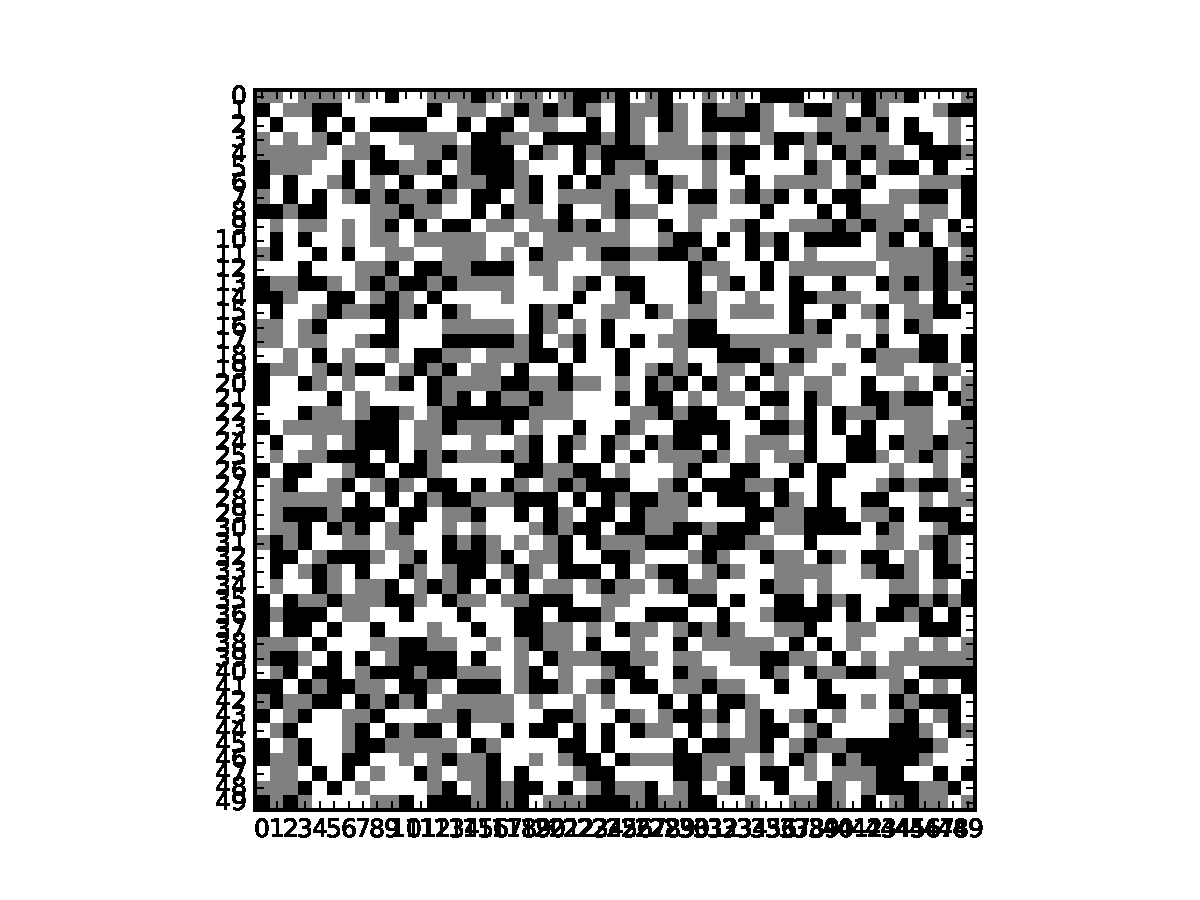
\includegraphics[width=\linewidth]{./Plots/lattice_0.pdf}
    \caption{At $t$ = 0}
  \end{subfigure}
  %
  \begin{subfigure}[b]{0.32\textwidth}
    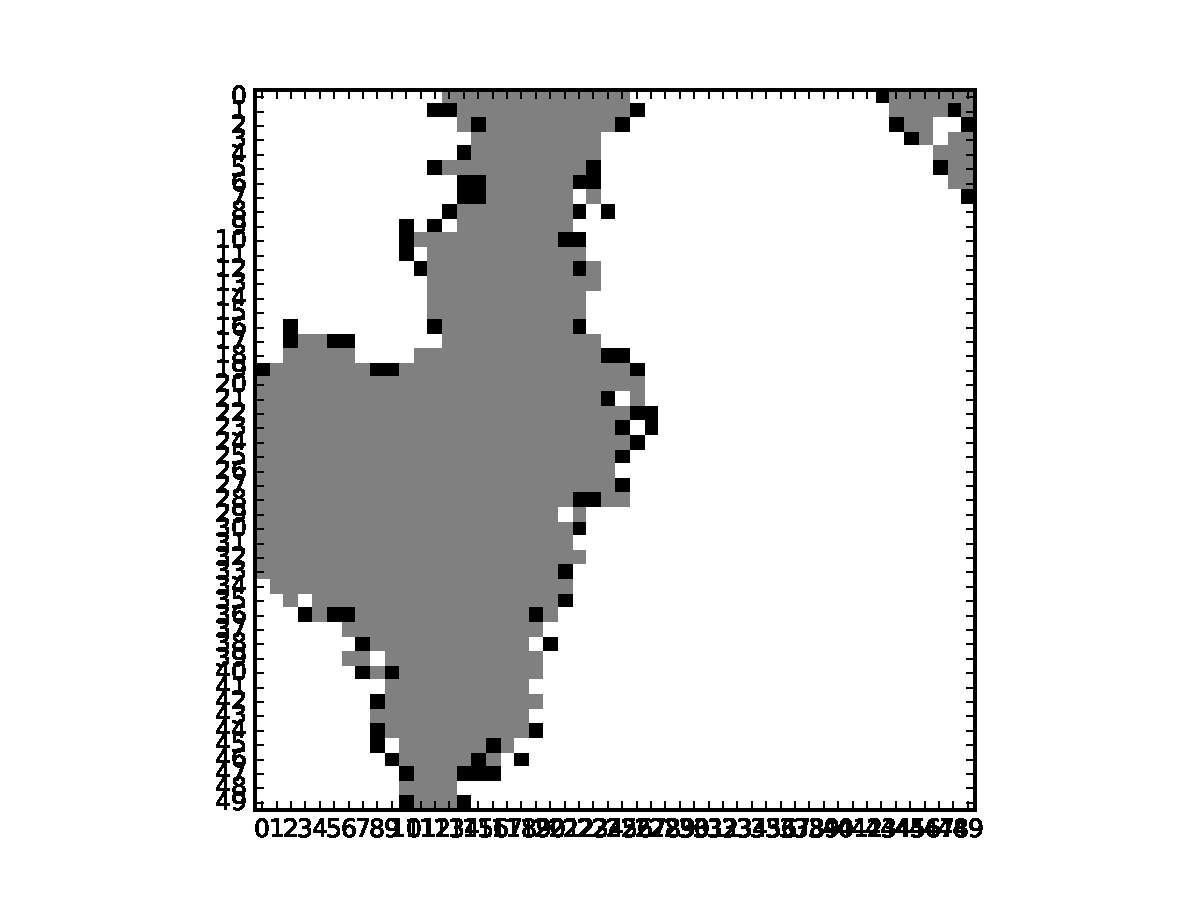
\includegraphics[width=\linewidth]{./Plots/lattice_500.pdf}
    \caption{At $t$ = 500}
  \end{subfigure}
 %
  \begin{subfigure}[b]{0.32\textwidth}
    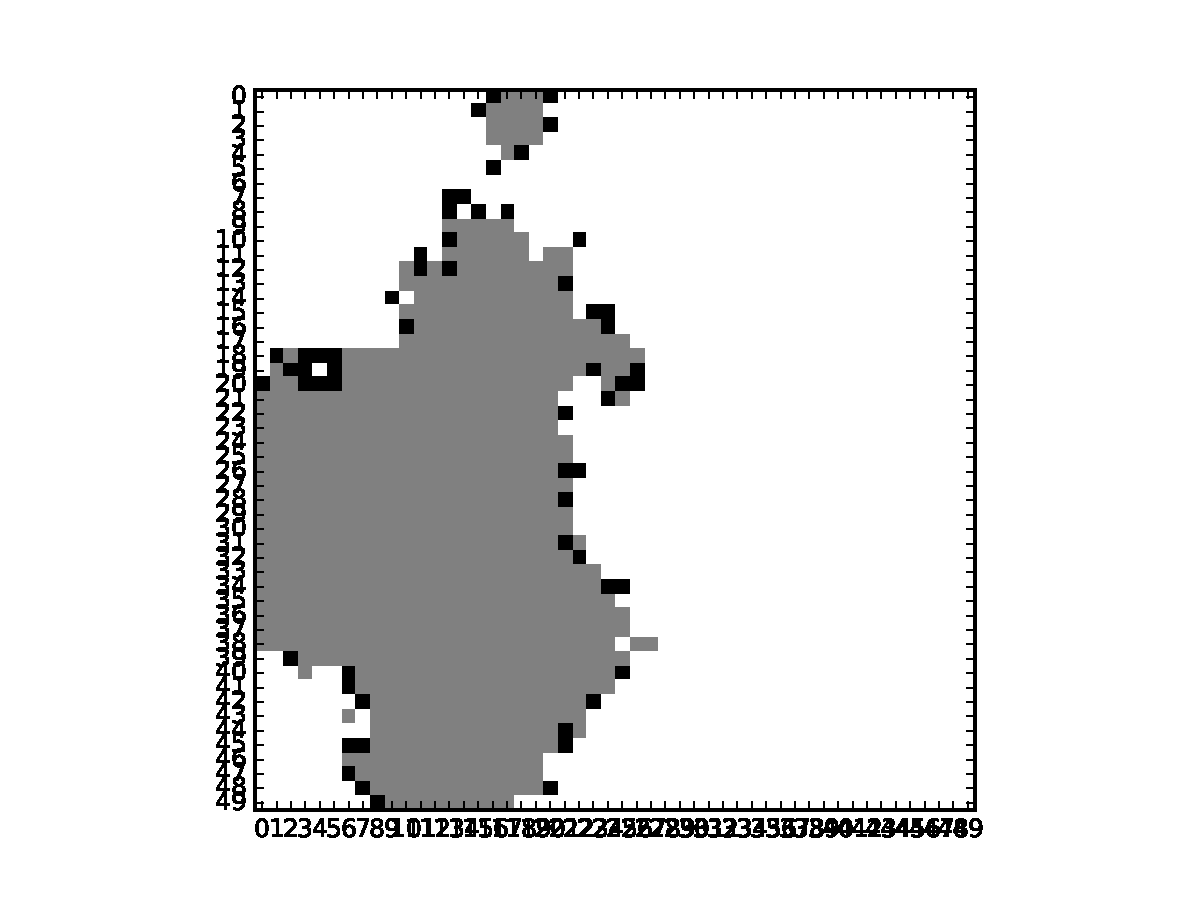
\includegraphics[width=\linewidth]{./Plots/lattice_1000.pdf}
    \caption{At $t$ = 1000}
  \end{subfigure}
\caption{Model of regular lattice for 2500 agents at $t$ = 0, 500 and 1000. White: language A users; Grey: language B users; Black: bilingual users}
\label{regular_lattice}
\end{figure}



The results of Erdos Renyi random network, small world network and scale-free network are similar and dominance of a language gradually occurs in these networks. Figure \ref{ohne_comm_ep} shows how percentage of agents in each state changes against number of iterations for the three networks. At the beginning, number of language A and language B users are the same. However, one of the languages quickly dominates when the number of agents in that monoligual state exceed that of the other. The simulation time required for dominance to occur are different but the outcomes are more or less the same. It is notable that one of the languages completely die out within 100 iterations in a scale-free network. The change in ratio is more rapid when compared with the results of the other two networks. 


\begin{figure}
  \begin{subfigure}[b]{0.32\textwidth}
    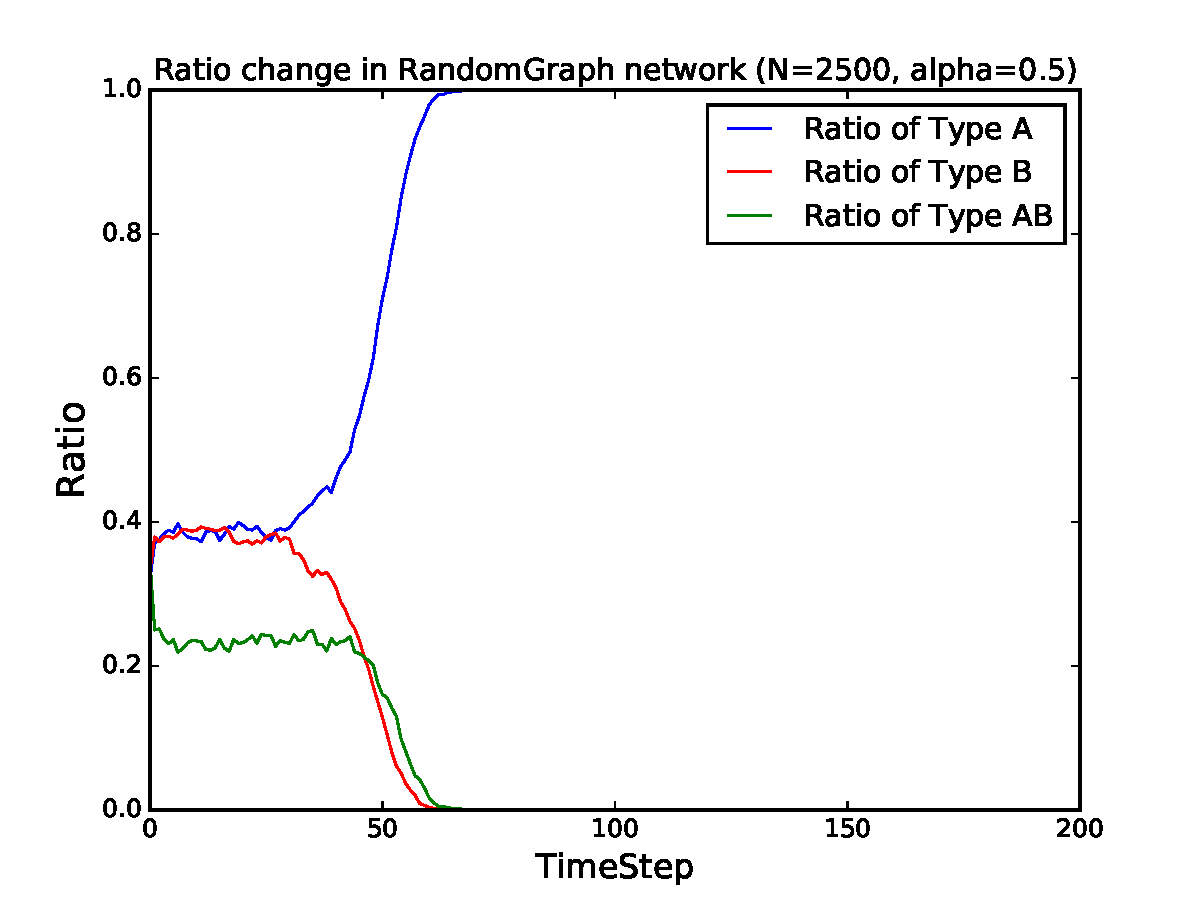
\includegraphics[width=\linewidth]{./Plots/Random_2500_0p5.pdf}
    \caption{Erdos Renyi random network}
  \end{subfigure}
  %
  \begin{subfigure}[b]{0.32\textwidth}
    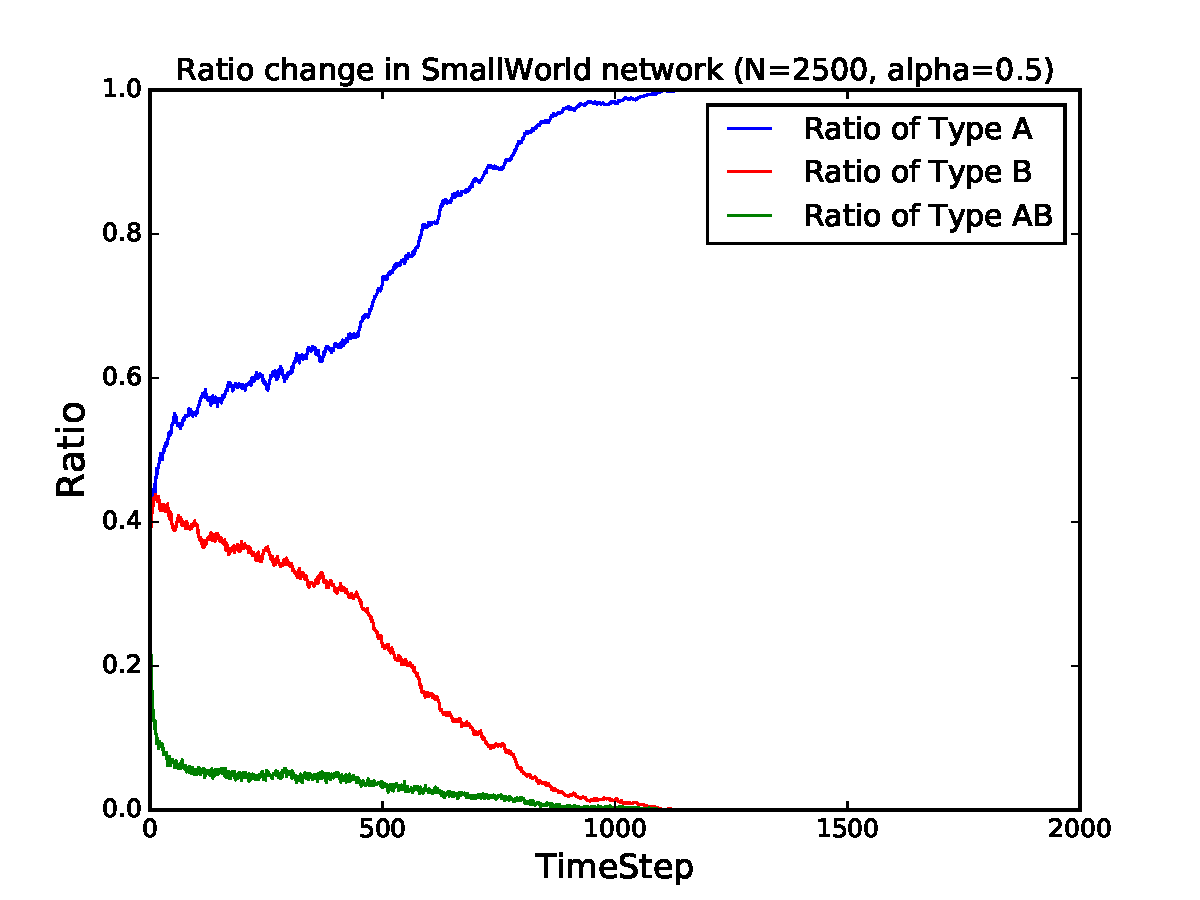
\includegraphics[width=\linewidth]{./Plots/SW_2500_0p5.pdf}
    \caption{Small world network}
  \end{subfigure}
 %
  \begin{subfigure}[b]{0.32\textwidth}
    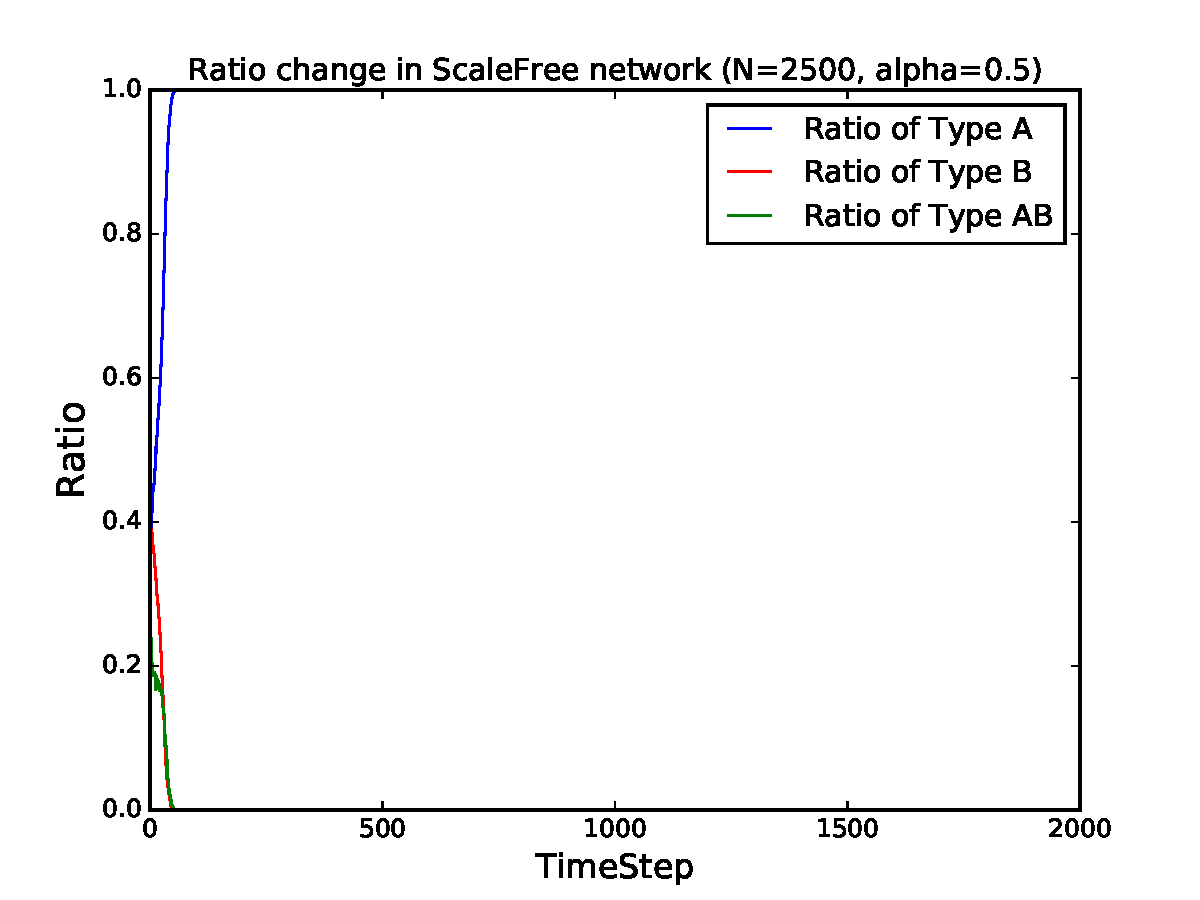
\includegraphics[width=\linewidth]{./Plots/SF_2500_0p5.pdf}
    \caption{Scale-free network}
  \end{subfigure}
\caption{Plots of percentage of agents in different states againt time for models with Erdos Renyi Random Network, small world network and scale-free network for 2500 agents. Prestige of both language is 0.5. Blue: language A users; Red: language B users; Green: bilingual users}
\label{ohne_comm_ep}
\end{figure}


The results do make sense. For instance, in the random network, where probability of having a tie is equal in the whole network, the density of a particular language use plays an important part. If density of language A users is greater than that of language B users at a certain part, it is almost certain that the density of A will keep on increasing until dominance occurs. In the small world network case, agents are closely connected and agents are able to reach all the other agents in a small number of steps. As a result, it makes sense that the usage of a language can be quickly spread within the society. As for the scale-free network, its degree distribution follows a power law, which means that the degrees are high for a few agents and most agents have low degree in the society. Those agents with high degree can easily influence those with low degree, as a result, agents rapidly switch to the same language state. 

In contrast, the social circle network, which resembles the community structure in a society, results in coexistence in the long run. In our example, we assume there are five Barabasi-Albert networks in a society with 2500 agents and each community is loosely and randomly connected to the other communities. The result, as shown in Figure \ref{social_circle}, meets our expectation. In comparison to the networks above, community structure seems to be essential to prevent or delay the occurance of a language dominace. The change in ratio is rapid at first and becomes stable after a small number of steps. We observe that agents quickly switch to the same language within the communities, and thus, results in the great change in the small time step. Furthermore, agents rarely change their states once their local communities have converged to the same language. However, we observe one peculiarity in the simulation. The starting model has equal number of language A and language B users, and they are situated randomly into different communities. We expect the resulting ratio of the two languages to be same, yet it turns out that majority, about 80\%, of the population switch to language B. This may be due to randomisation. As said before, the the coexistance of both languages is very unstable and the final state is greatly influenced by the initialisation. Because of the random initialisation, it is likely that 4 communities end up speaking language B and the other one speaking language A, which is shown in Figure \ref{social_circle} and \ref{comm_noiseEdge}.%\textcolor{red}{-explain further}

\begin{figure}[!tbp] 
  \centering
  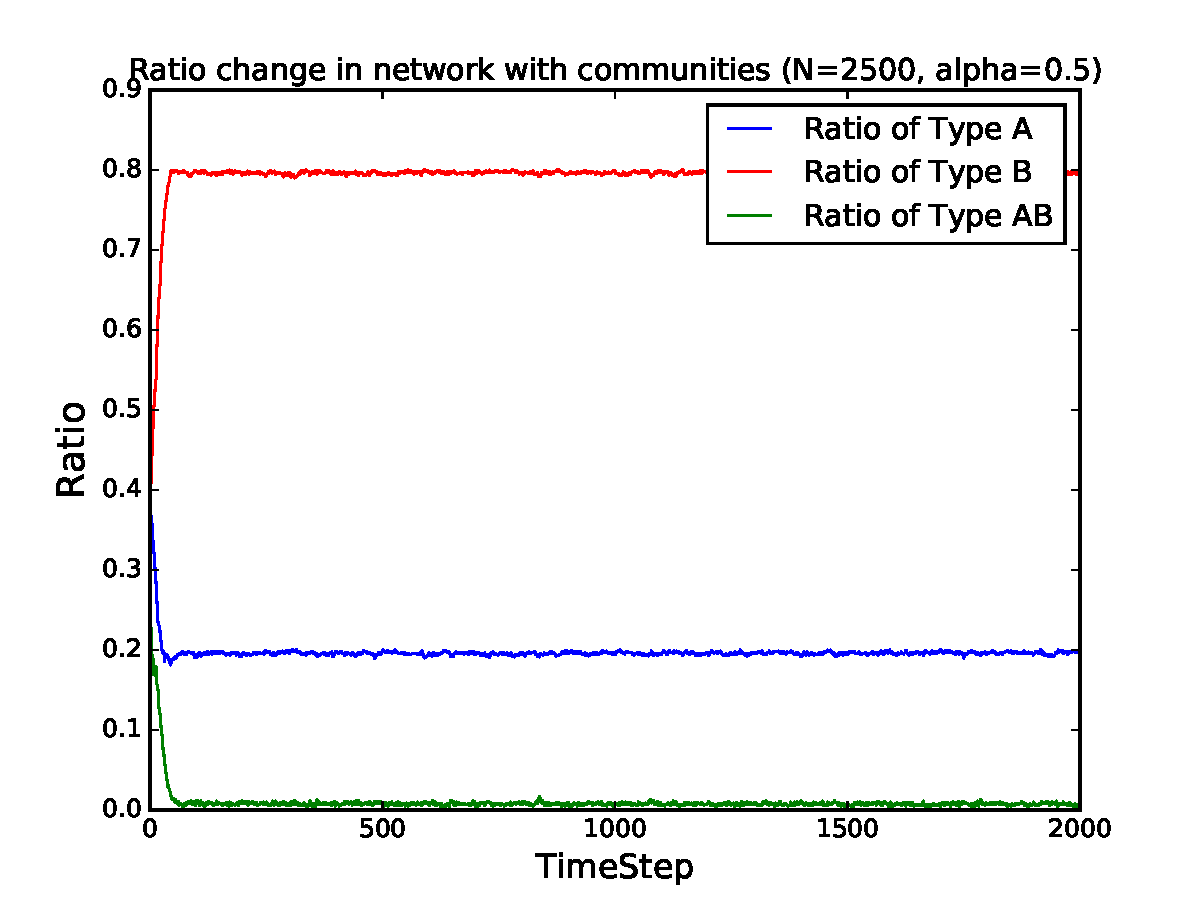
\includegraphics[width=80mm, scale=0.6]{./Plots/com_2500_0p5.pdf}
\caption{Plots of percentage of agents in different states againt time for models with social circle network for 2500 agents.}
\label{social_circle}
\end{figure}



\begin{figure}
  \begin{subfigure}[b]{0.32\textwidth}
    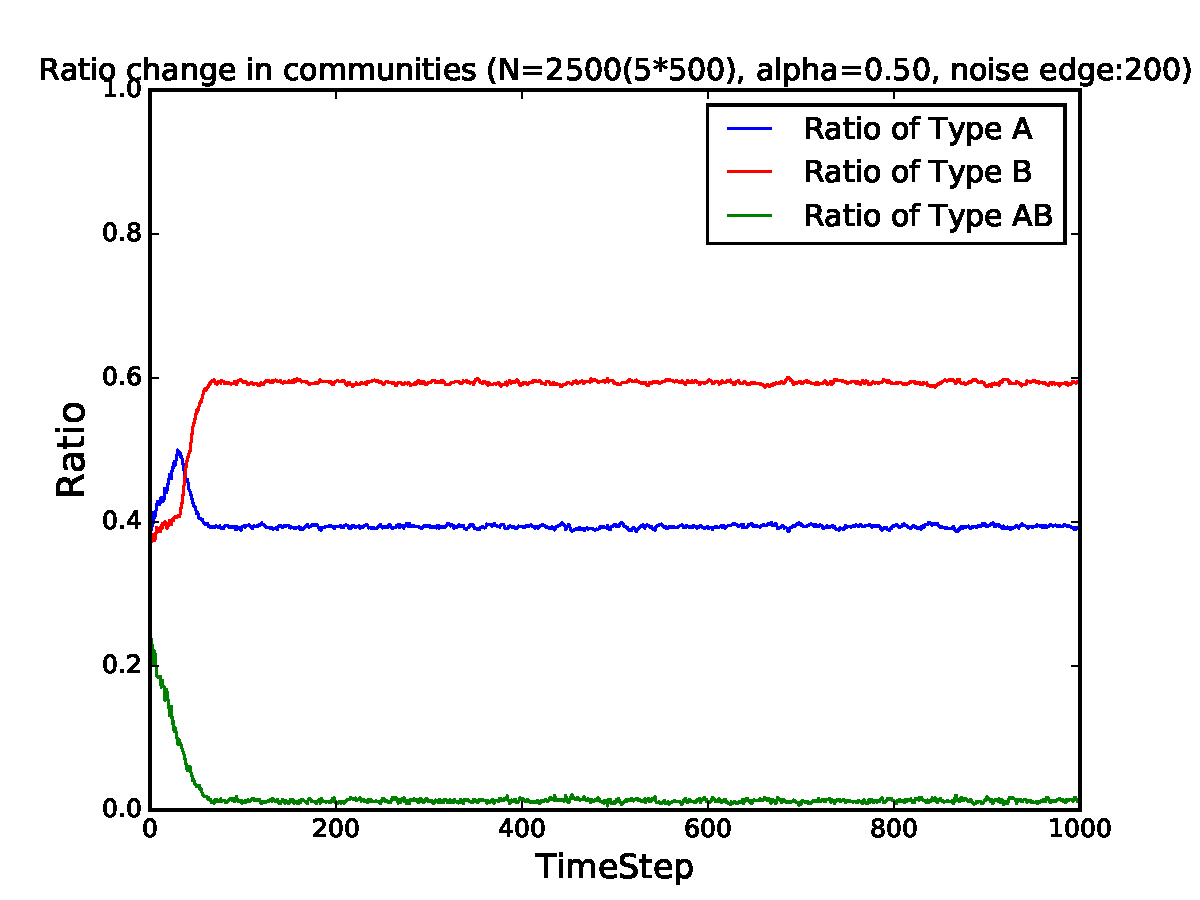
\includegraphics[width=\linewidth]{./Plots_new/com_5_0p5_200.pdf}
    \caption{200 intra edges}
  \end{subfigure}
  %
  \begin{subfigure}[b]{0.32\textwidth}
    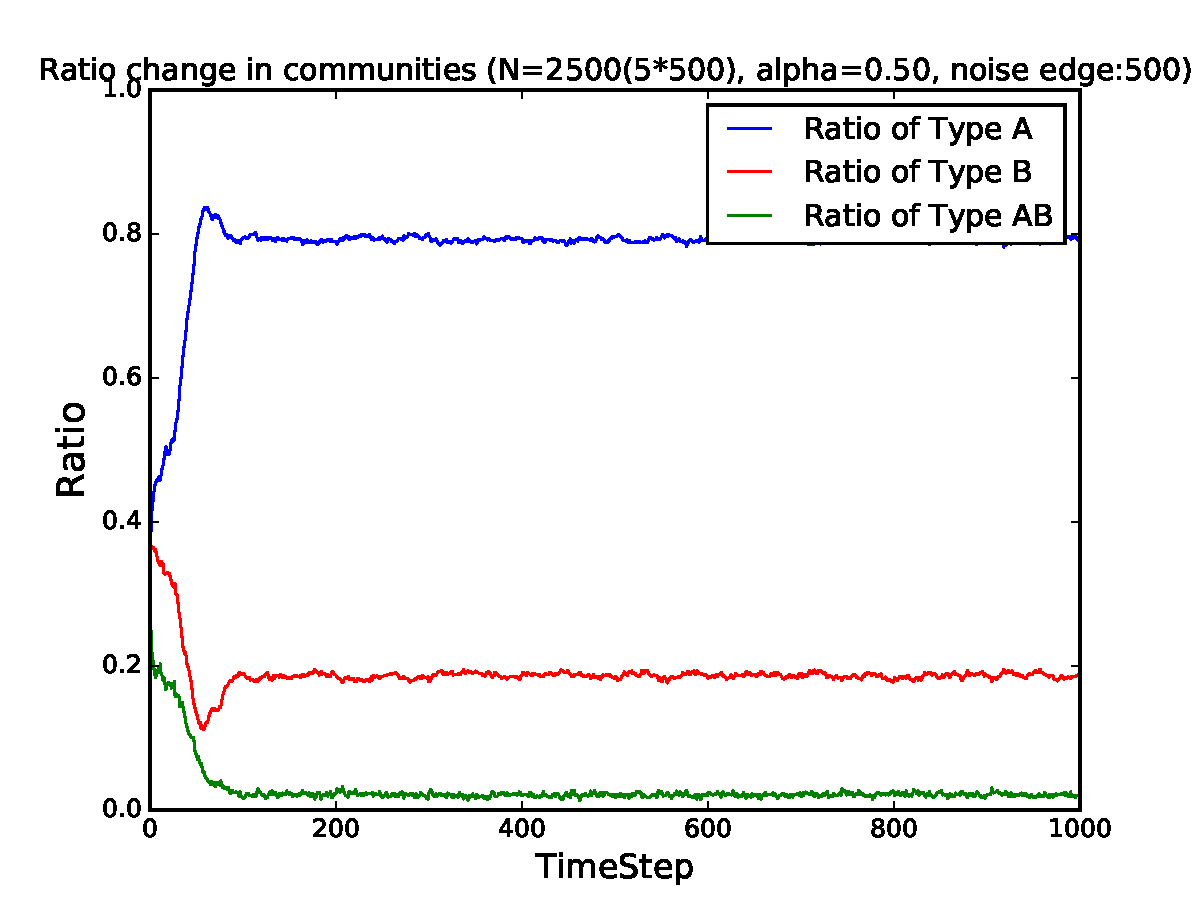
\includegraphics[width=\linewidth]{./Plots_new/com_5_0p5_500.pdf}
    \caption{500 intra edges}
  \end{subfigure}
 %
  \begin{subfigure}[b]{0.32\textwidth}
    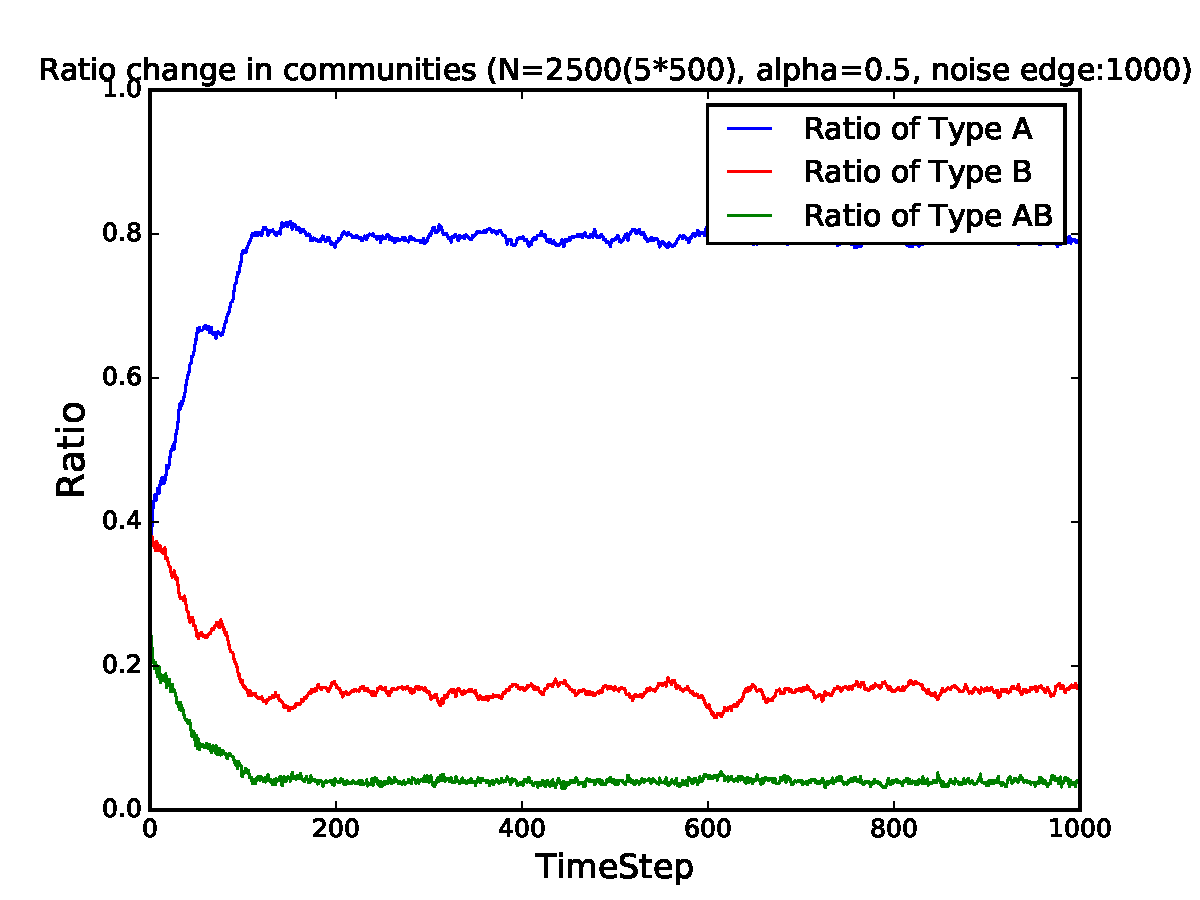
\includegraphics[width=\linewidth]{./Plots_new/com_5_0p5_1000.pdf}
    \caption{1000 intra edges}
  \end{subfigure}
\caption{Plots of percentage of agents in different states againt different noise edges with social circle network for 2500 agents. The edges between different communities are 200, 500 and 1000.}
\label{comm_noiseEdge}
\end{figure}

\section{Extension}
The simulation above are all produced under the assumption that the two languages are equally important. The community structure is able to withhold dominance of one group. The next question in mind is whether the effectiveness of the community structure remains strong when we alter the intial prestige of both languages, i.e. one language is more important than the other. 

First, we observe that dominance of a language will occur sooner if the prestige of a language is higher than the other for networks without community structure. Figure \ref{ohne_comm_up} shows that the number of agent in state A increases rapidly when the prestige of language A increases from 0.5 to 0.55. Small change in prestige seems to have great effect already. 

\begin{figure}
  \begin{subfigure}[b]{0.32\textwidth}
    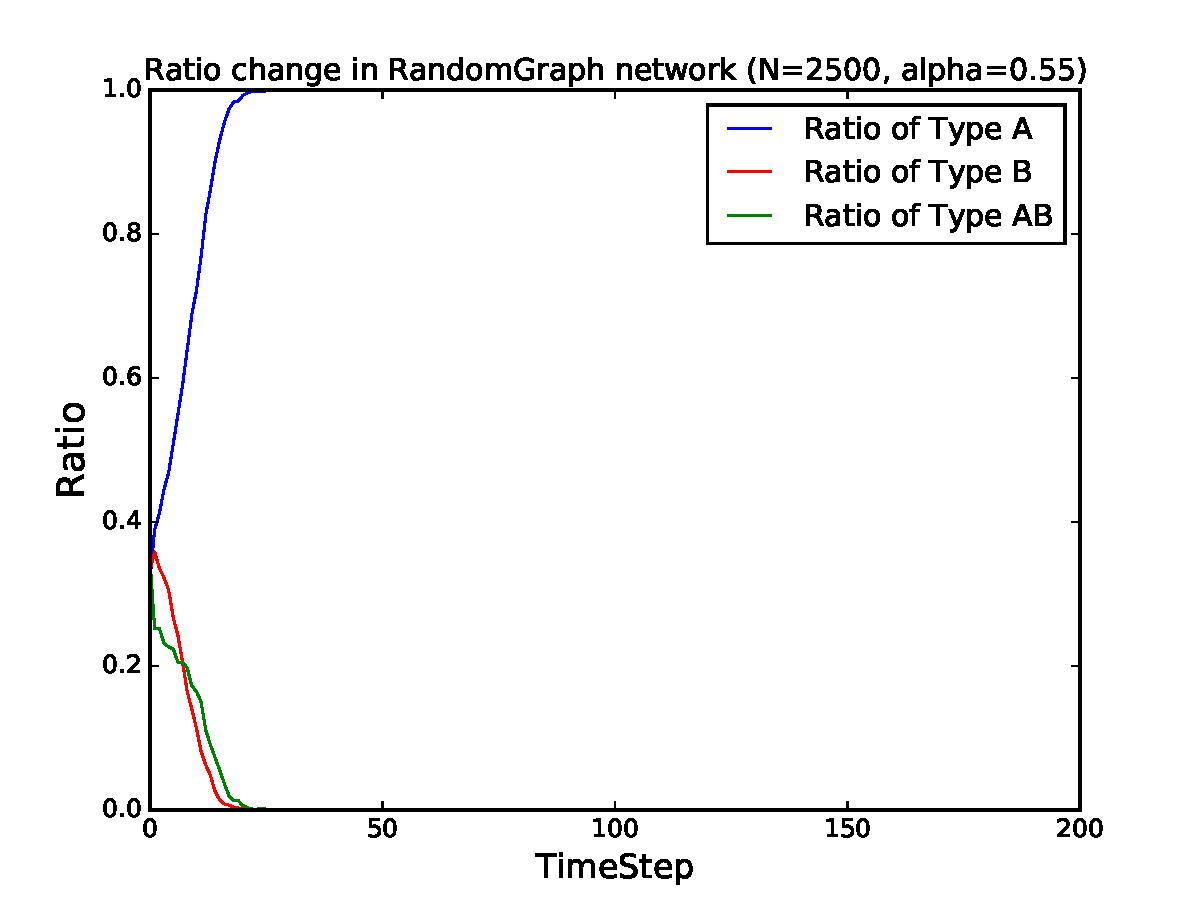
\includegraphics[width=\linewidth]{./Plots/Random_2500_0p55.pdf}
    \caption{Erdos Renyi random network}
  \end{subfigure}
  %
  \begin{subfigure}[b]{0.32\textwidth}
    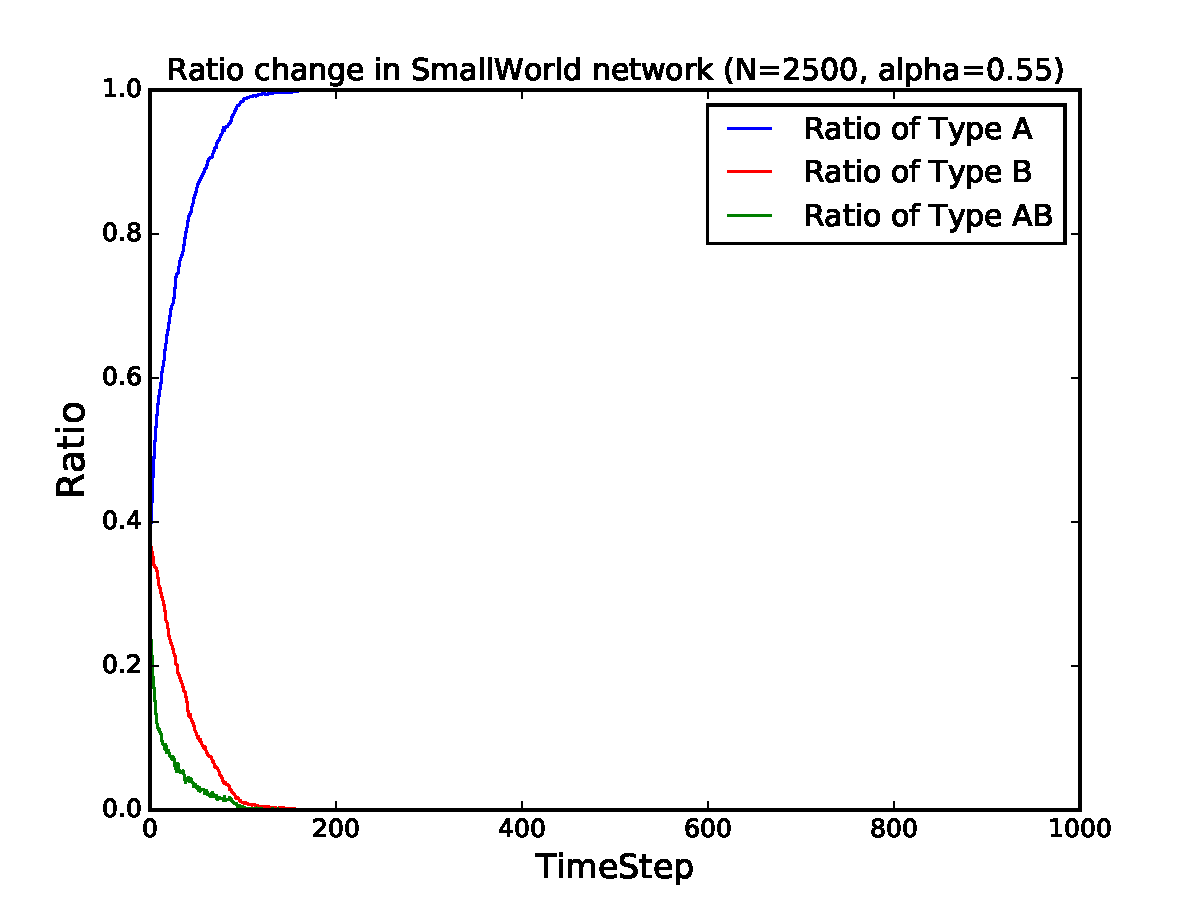
\includegraphics[width=\linewidth]{./Plots/SW_2500_0p55.pdf}
    \caption{Small world network}
  \end{subfigure}
 %
  \begin{subfigure}[b]{0.32\textwidth}
    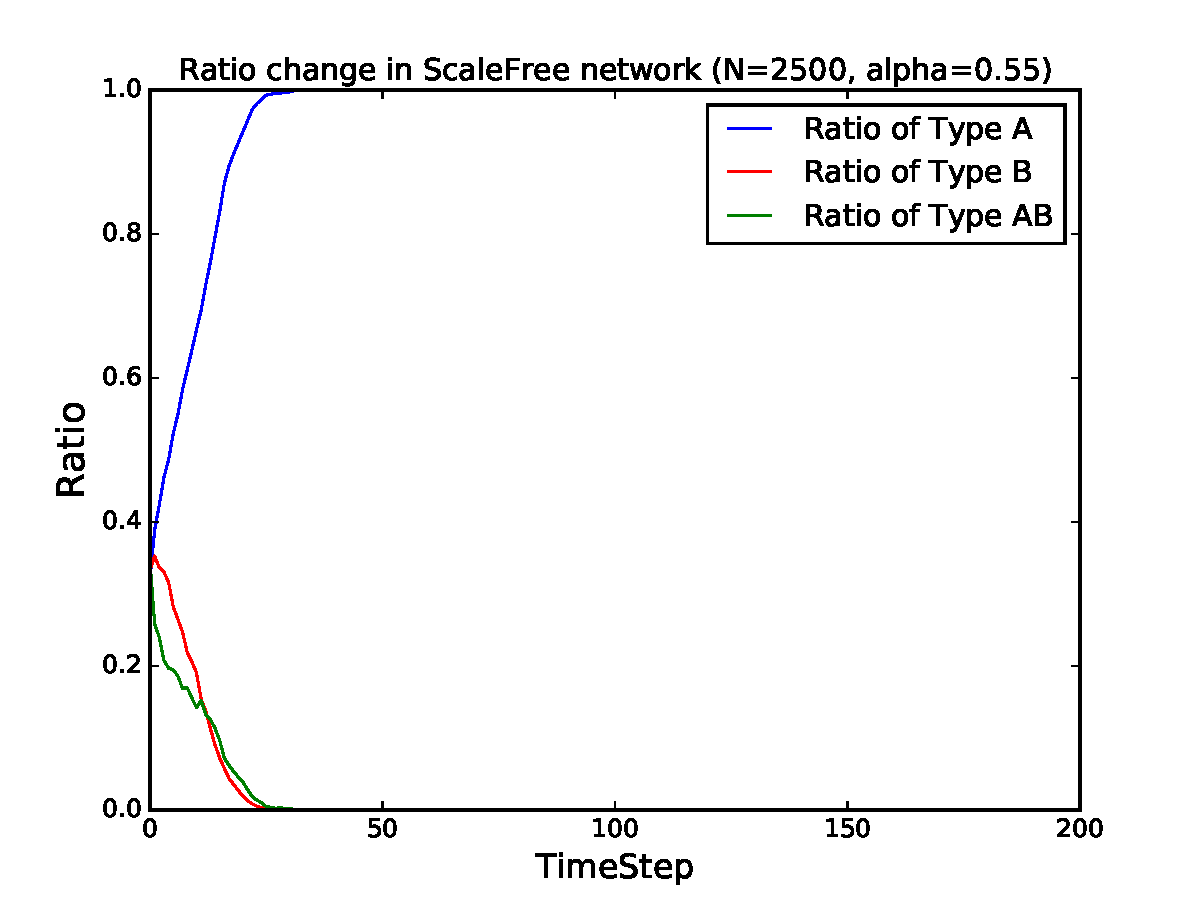
\includegraphics[width=\linewidth]{./Plots/SF_2500_0p55.pdf}
    \caption{Scale-free network}
  \end{subfigure}
\caption{Plots of percentage of agents in different states againt time for models with Erdos Renyi Random Network, small world network and scale-free network for 2500 agents. Prestige of language A is 0.55. Blue: language A users; Red: language B users; Green: bilingual users}
\label{ohne_comm_up}
\end{figure}

We then experiment the effects of prestige in social circle network. As shown in Figure \ref{social_circle_up}, the community structure can still withhold the effect of prestige and both language states coexist when the prestige parameter $\alpha$ is increased slightly. However, it cannot withhold the effect of prestige when the prestige goes up to 0.55. 

\begin{figure}[!tbp] 
  \centering
  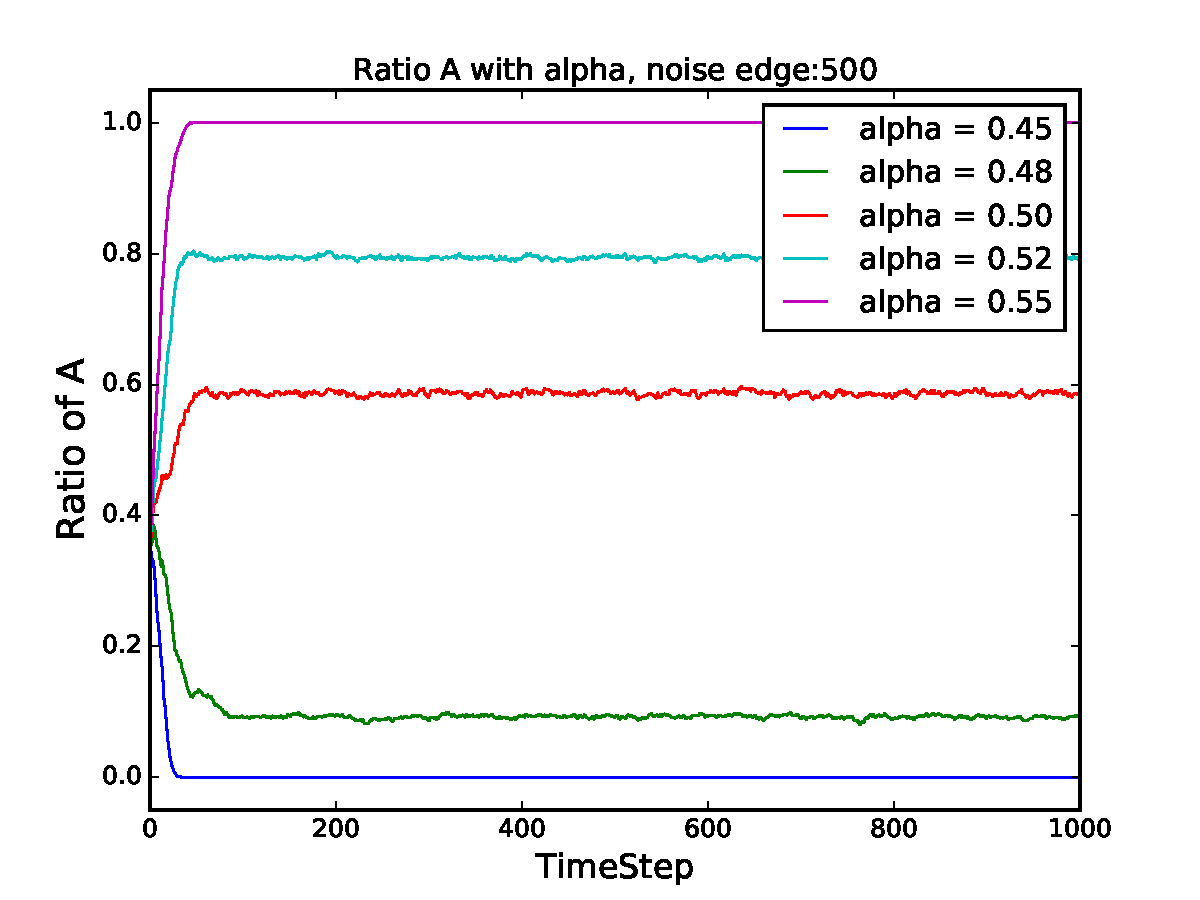
\includegraphics[width=80mm, scale=0.6]{./Plots_new/RatioA_withAlpha_500.pdf}
\caption{Plots of percentage of agents in language state A againt time for models with social circle network for 2500 agents with $\alpha = \{0.45, 0.48, 0.50, 0.52, 0.55\}$. At beginning, the possibility for each agent to choose initial state is equal.}
\label{social_circle_up}
\end{figure}

Result shows that a more superior language has higher chance to dominate within a community, and as a result, dominates the whole society. This result is plausible. However, even though we expect that the inferior language will eventually become extinct, this phenomenon is too sensitive to language prestige and occurs sooner than what we first expect. Community structure seems have little influence to wane the effect of unequal prestige of the two languages. 


\begin{figure}[!tbp] 
  \centering
  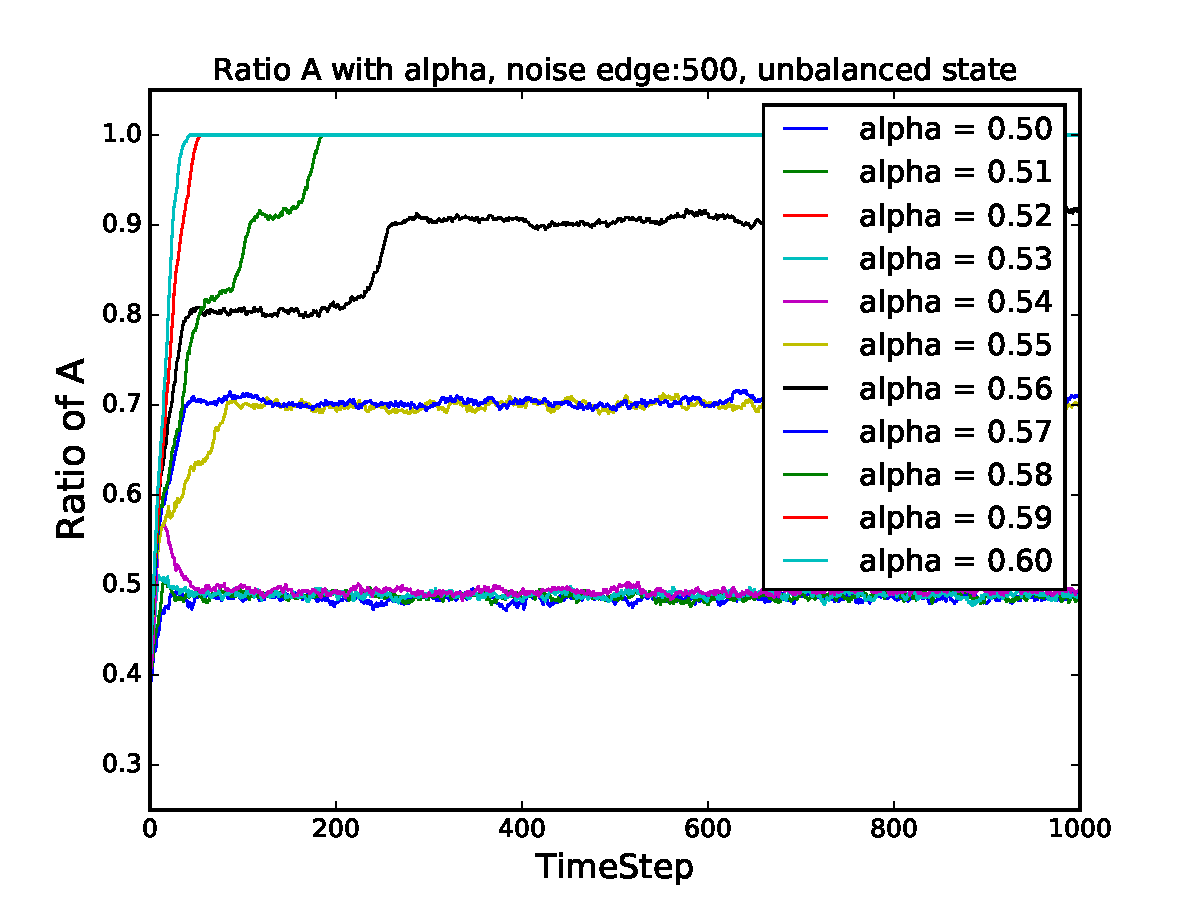
\includegraphics[width=80mm, scale=0.6]{./Plots_new/RatioA_withAlpha_500_unbalanced2.pdf}
\caption{Plots of percentage of agents in language state A againt time for models with social circle network for 2500 agents with $\alpha \in [0.50, 0.60]$. }
\label{comm_unbalance}
\end{figure}

However, we realise that, for each agent, the possibility of choosing states at beginning could be different. Up to now, each agent has the same possiblility to language A and language B at beginning. However, it is more possible that the majority in different communities speaks different languages. So we set different initial possibility in different communities. In Figure \ref{comm_unbalance}, there are ten communities in total. In five communities, the possibilies for each agent to be A, B and AB at beginning are 0.70, 0.25 and 0.05 respectively. In the other five communities, the possibilies for each agent to be A, B and AB at beginning are 0.25, 0.70 and 0.05 respectively. As shown in Figure \ref{comm_unbalance}, the coexistence could still exist when A's prestige goes up to 0.56. This is because the effect of language A's prestige could be waned if most people speak B at beginning and vice versa. So the final state is less sensitive to language prestige when different communities have different major languages. This result shows us that the outcome is influenced by both the structure of communities as well as the composition within each community. 

\section{Conclusion}

As shown in above section, community structure is an important factor for coexistance of two equally important languages. However, the strength of this structure is sensitive to the prestige parameter we set. We expect greater tolerance against the effect of prestige for model with community structure, yet dominance is bound to happen when the prestige parameter is above 0.55 in our trial. Nonetheless, community structure is undeniably an important factor which affects the way two languages come together in a society. And, the dominance could be further waned when communities have different superior languages at beginning.

The networks we selected only reflect some particular features of agents' interactions in a society. Hence, it is not realistic to interpret the real situation from just one particular network. Even though the social circle network reflects the community structure we are most interested, one should not ignore other features described in other networks. For example, a scale-free network or a small world network may represent better how information flows in a society.  Certainly, a social network in reality is a mixture of all the selected networks. One may examine further by considering a network that has combined features. 

Besides, one may improve the randomisation further in the design of the community structure. This is because one may find our design of the community structure somewhat rigid as the number of agents in each community is the same and expect more connections between communities in reality. Despite of that, we believe our models are sufficient to descibe the basic features in a language competition model, and it provides a good foundation for further exploration.

\bibliography{ref}{}
\bibliographystyle{plain}

\end{document} 

%%% Local Variables:
%%% mode: latex
%%% TeX-master: t
%%% End:
